\lstinputlisting[language=bash,basicstyle=\small]{python_codes/fieldstone_70/keywords}

\begin{center}
Code at \url{https://github.com/cedrict/fieldstone/tree/master/python_codes/fieldstone_70}
\end{center}

\par\noindent\rule{\textwidth}{0.4pt}

%%%%%%%%%%%%%%%%%%%%%%%%%%%%%%%%%%%%%%%%%%%%%%%%%%%%%%%%%%%%%%%%%%%%%%%%%%%%%%%%%%%%%%%%%%%%%%%%%%%%

The setup is borrowed from Duretz et al (2020) \cite{dudy20}. 
Two major differences with the paper: 1) no elasticity and 2) no Newton solver.

The model consists of a $100\times 30$km slice of Westerly Granite (Hansen \& Carter, 1983), 
which comprises an imperfection at the center of the domain.
This weak inclusion with a 2 km radius serves to initiate
localized deformations. The model configuration is thus perfectly symmetric. 
The model includes a vertical temperature gradient ($-15\degree$C/km) (starting 
at $20\degree$C at the surface), 
a constant density (2700 kg/m$^3$), and the acceleration of gravity ($g_y=-10$m/s$^2$).
The inclusion is characterrised by $\eta=10^{20}\text{Pa}\cdot \text{s}$.
The domain is subjected to kinematic boundary conditions, which cause a pure shear stress
state:

\begin{center}
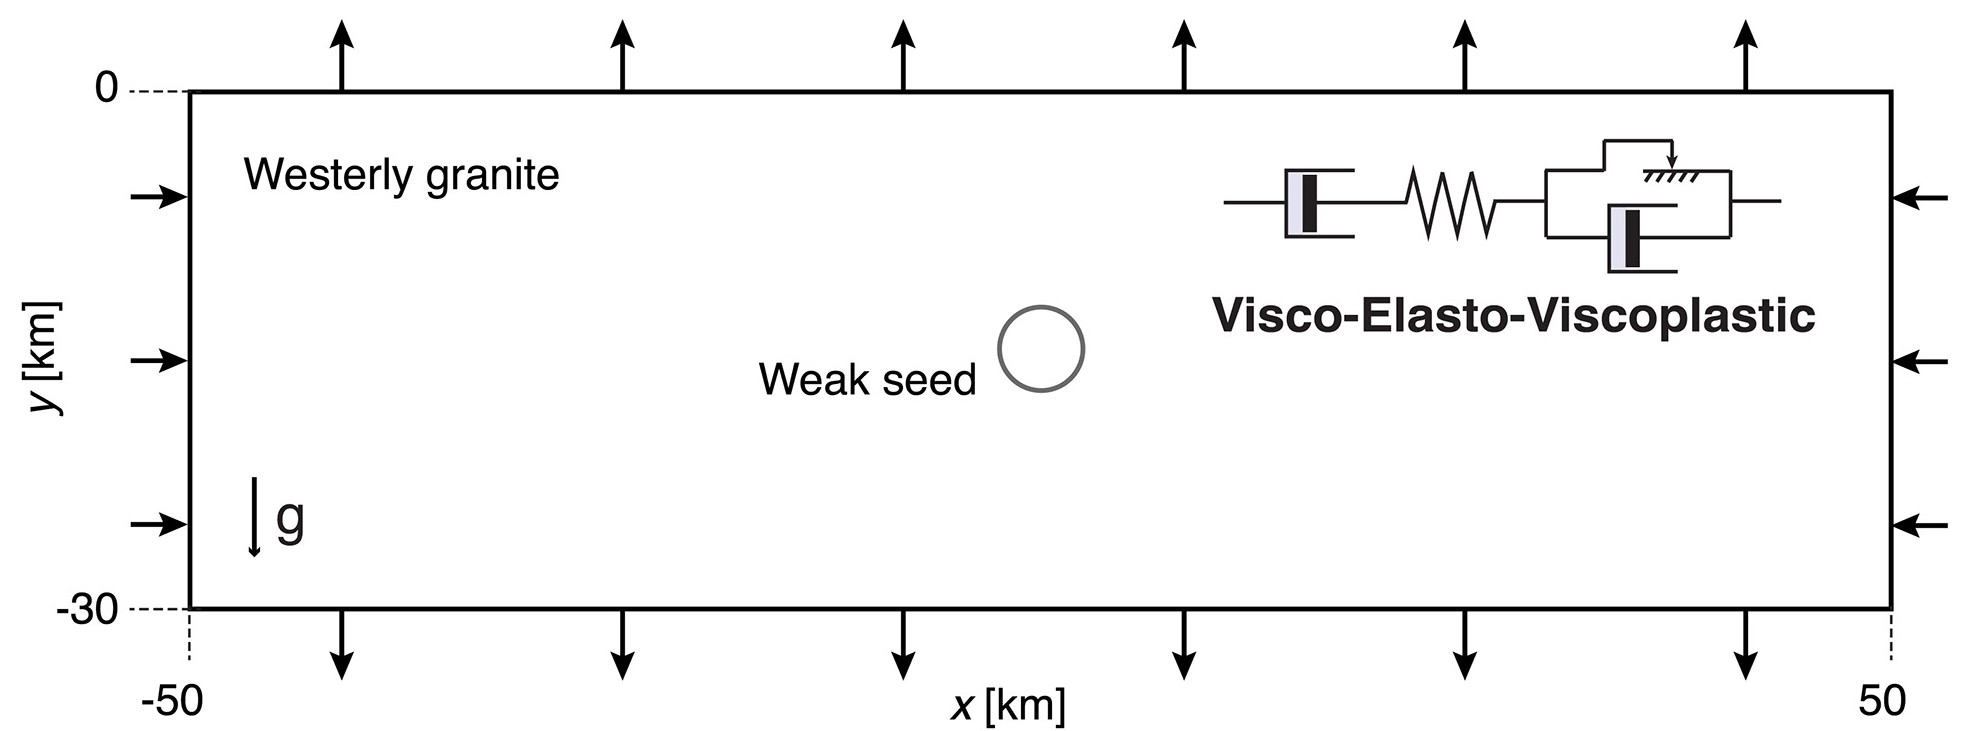
\includegraphics[width=12cm]{python_codes/fieldstone_70/images/fig1}\\
{\captionfont Figure taken from \cite{dudy20}}
\end{center}

All boundaries are free slip. The material can behave in a ductile manner in the lower, hot
part of the domain (displaying temperature-dependent power law creep), and in a viscoplastic 
manner in the upper, cold part of the domain. 
The parameters are 
$A=3.1623\cdot 10^{-26}\text{Pa}^{-n}\cdot\text{s}^{-1}$, $Q=186.5\cdot 10^3 \text{J/mol}$, 
$n=3.3$, $c=50$MPa, $\phi=\arctan(0.6)\simeq 31\degree$ and $\eta^{vp}=10^{21}\text{Pa}\cdot\text{s}$. 

The background strainrate is set such that $\dot{\varepsilon}_{bc}=10^{-15}s^{-1}$, i.e. 
$v_{bc}=\pm \dot{\varepsilon}_{bc} L_x/2 $ on the sides and $v=\pm \dot{\varepsilon}_{bc} L_y/2 $
on the top and bottom boundaries.
Pressure is normalised such that it is on average zero on the top boundary. 
Picard iterarions are used. The 2-norm of the non-linear residual 
is monitored, as well as the following quantities ($i$ and $i-1$ are two consecutive nonlinear iterations):
\[
\xi_u = \frac{\|u^i-u^{i-1}\|_2}{ \|u^i+u^{i-1}\|_2}
\qquad
\qquad
\xi_v = \frac{\|v^i-v^{i-1}\|_2}{ \|v^i+v^{i-1}\|_2}
\qquad
\qquad
\xi_p = \frac{\|p^i-p^{i-1}\|_2}{ \|p^i+p^{i-1}\|_2}
\] 
 

The effective viscosity at every quadrature point is computed as follows:
\[
\eta_{eff} = \left( \frac{1}{\eta_{eff,v}}  + \frac{1}{\eta_{eff,vp}}  \right)^{-1}
\]
with 
\[
\eta_{eff,v} = A^{-1/n} \dot{\varepsilon}^{-1+1/n} \exp \frac{Q}{nRT}
\qquad
\text{and}
\qquad
\eta_{eff,vp} = \frac{p \sin \phi + c \cos \phi}{2 \dot{\varepsilon}}  + \eta_{vp}
\]
For the first nonlinear iteration there is no pre-existing velocity or pressure field so 
I set $\dot{\varepsilon}=10^{-15}$ in the viscosity function, 
just so that the rheological model does not explode. 
The viscosity is also maintained between $\eta_{min}=10^{19}\text{Pa}\cdot\text{s}$ 
and $\eta_{max}=10^{25}\text{Pa}\cdot\text{s}$.


\begin{center}
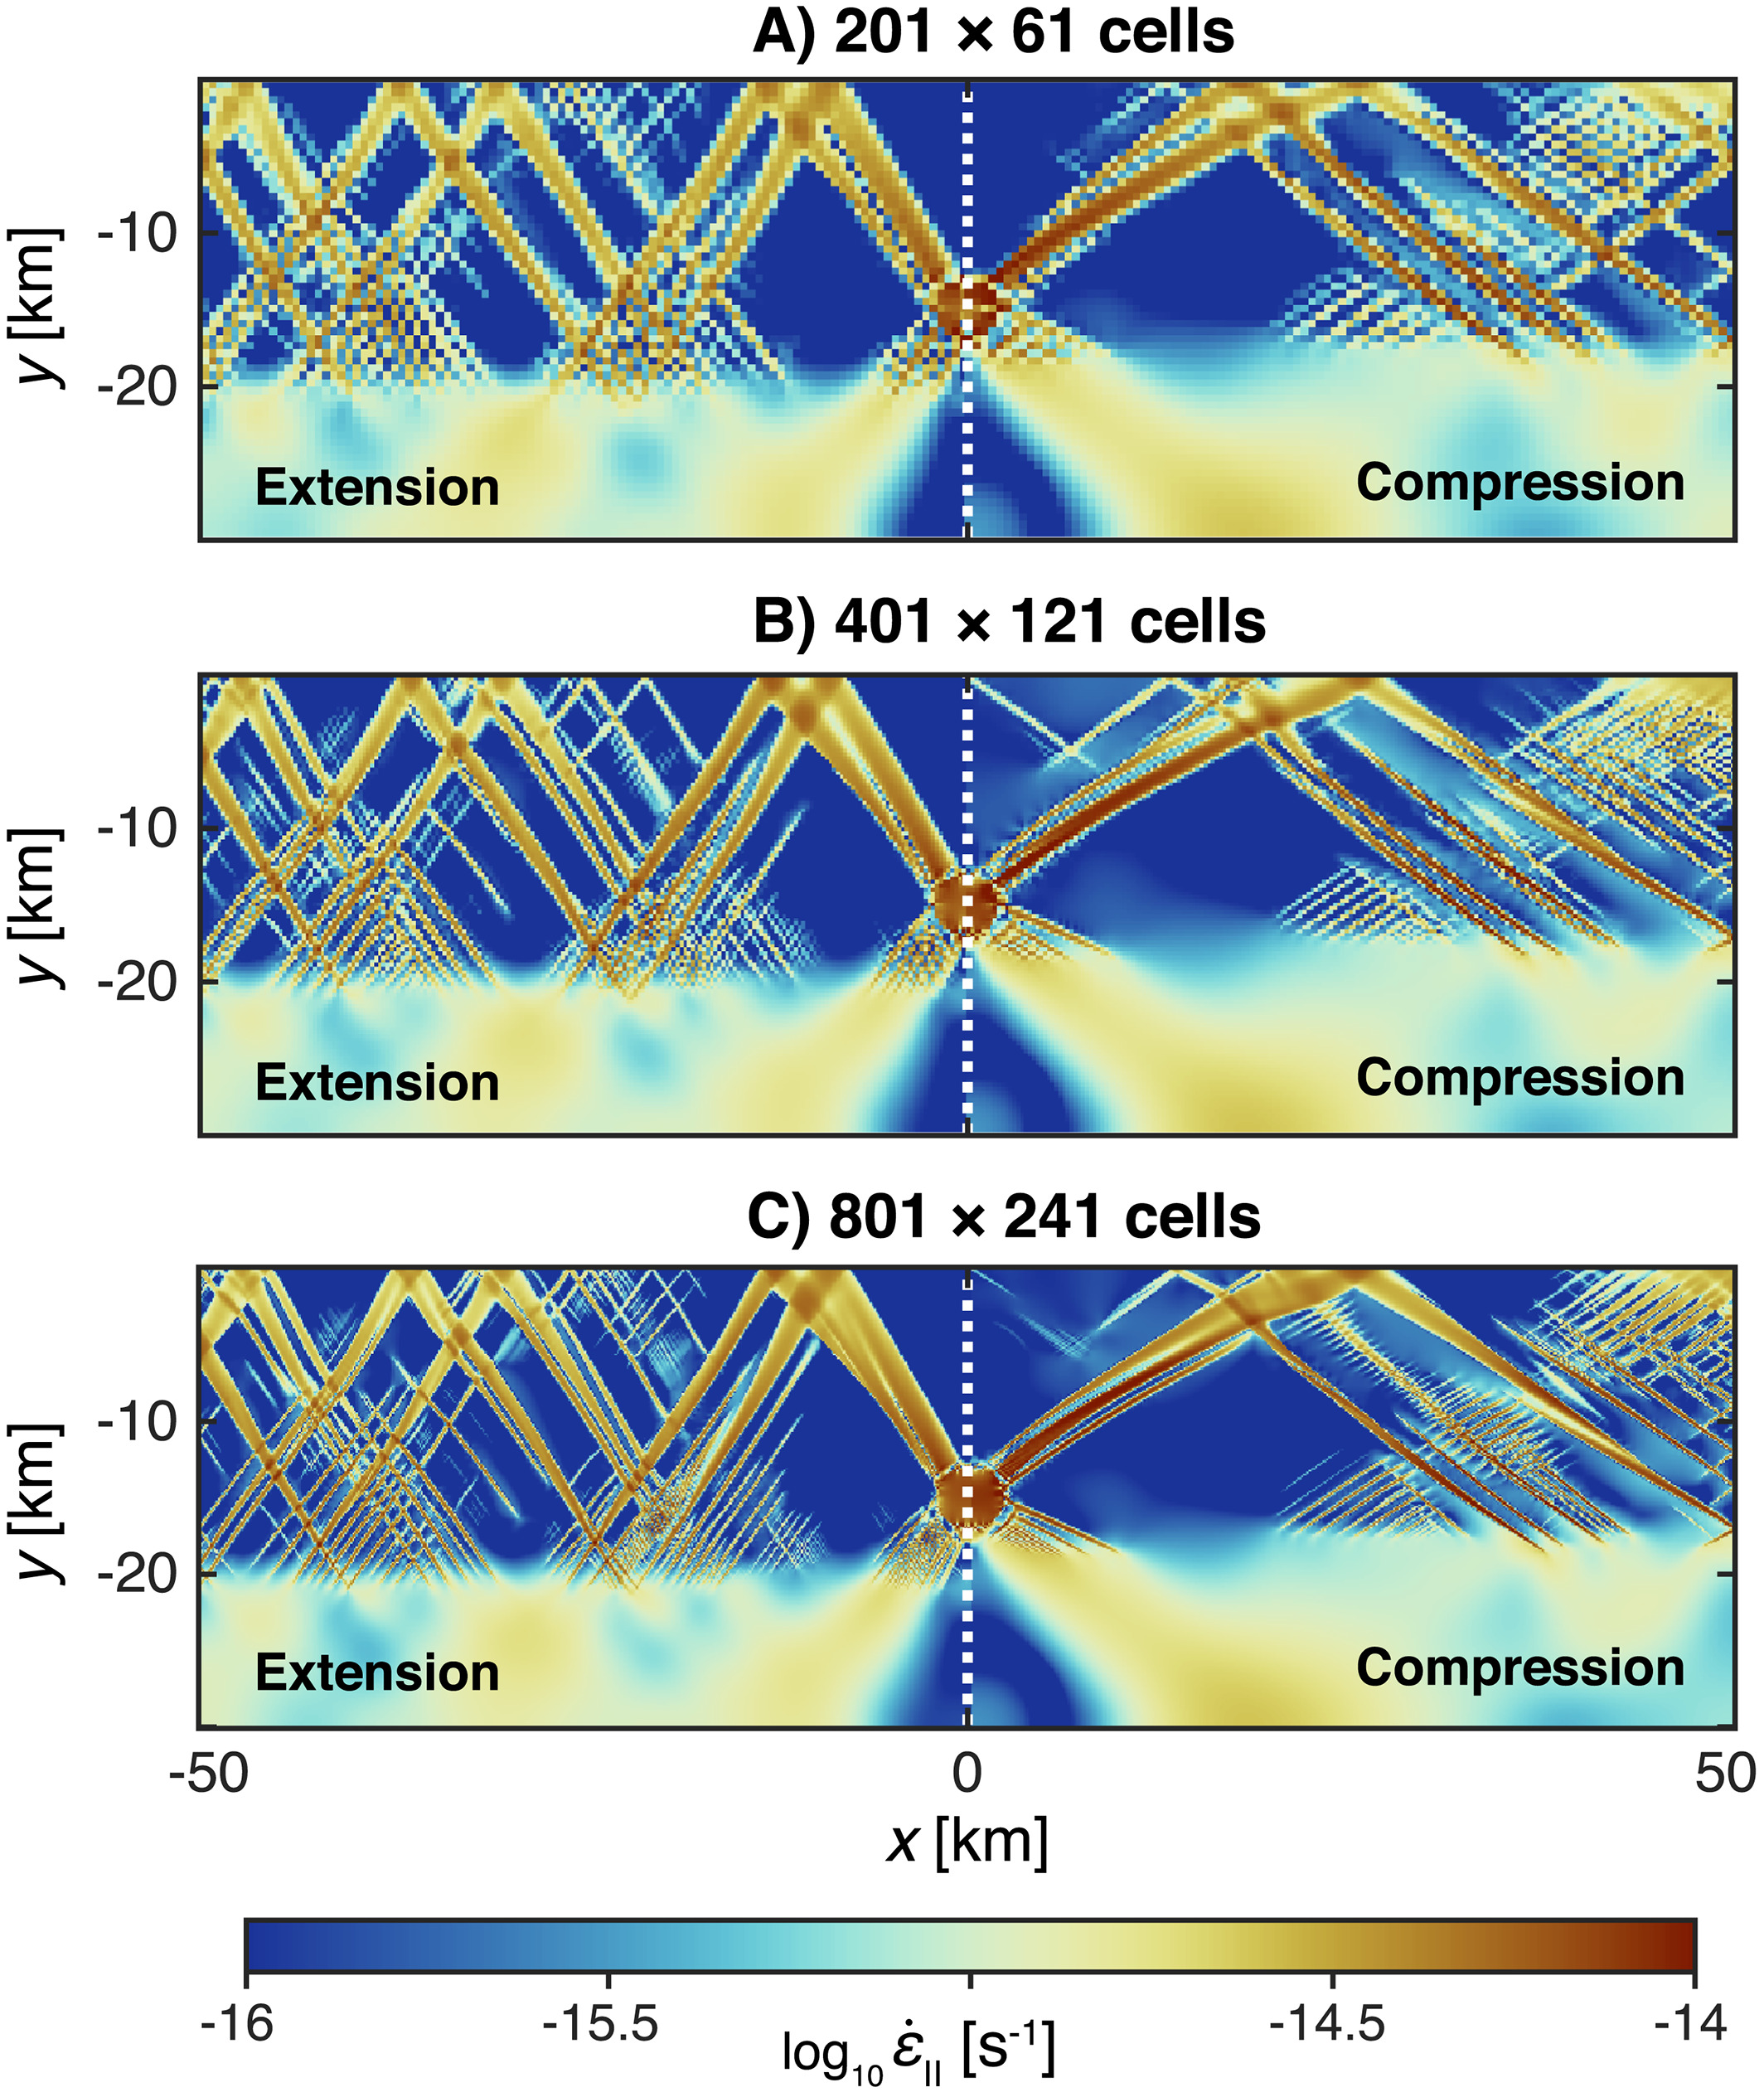
\includegraphics[width=13cm]{python_codes/fieldstone_70/images/fig2}\\
{\captionfont Figure taken from \cite{dudy20}}
\end{center}

explain tau plots

\newpage
%......................
\paragraph{Extension}.

\begin{center}
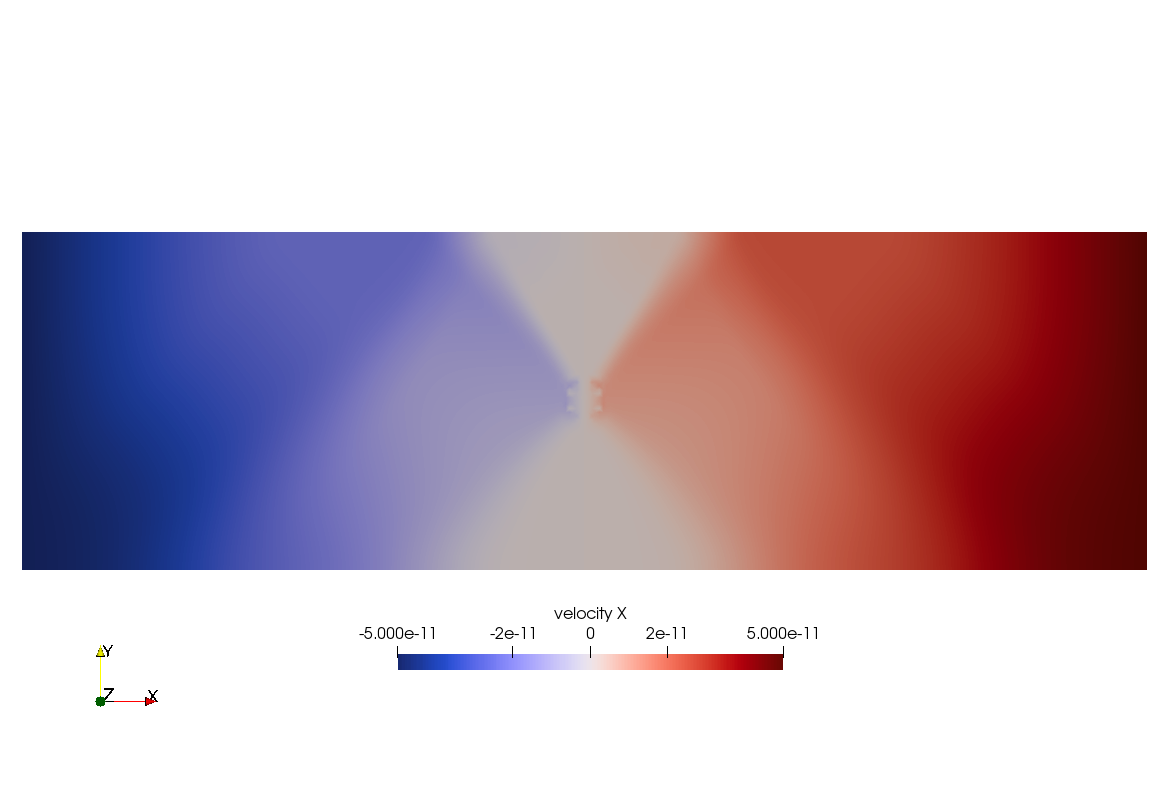
\includegraphics[width=7cm]{python_codes/fieldstone_70/extension/u}
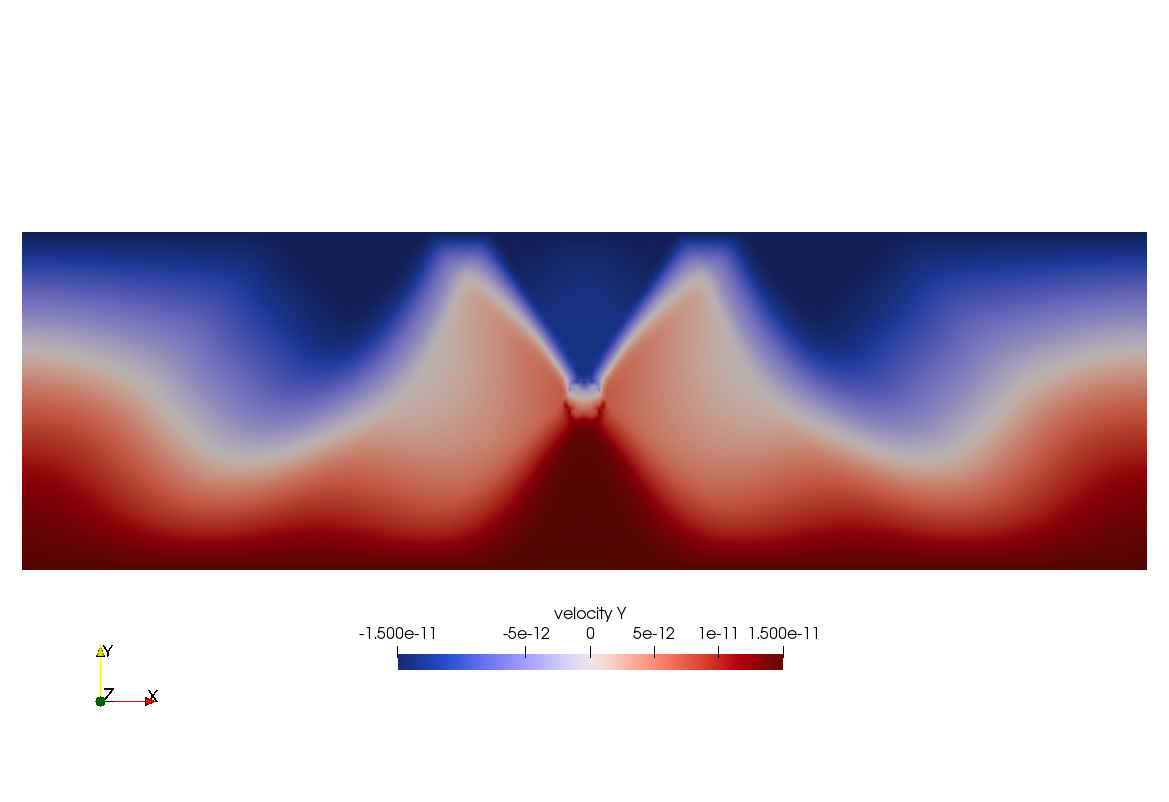
\includegraphics[width=7cm]{python_codes/fieldstone_70/extension/v}\\
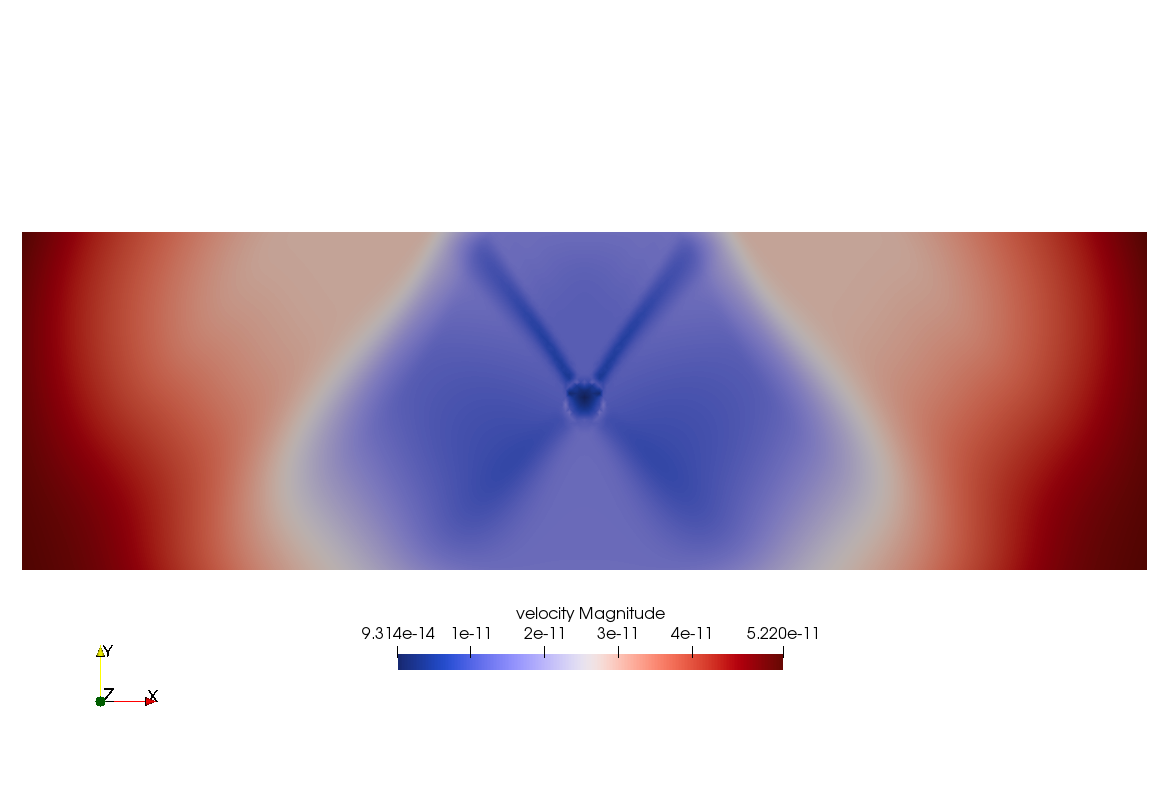
\includegraphics[width=7cm]{python_codes/fieldstone_70/extension/vel}
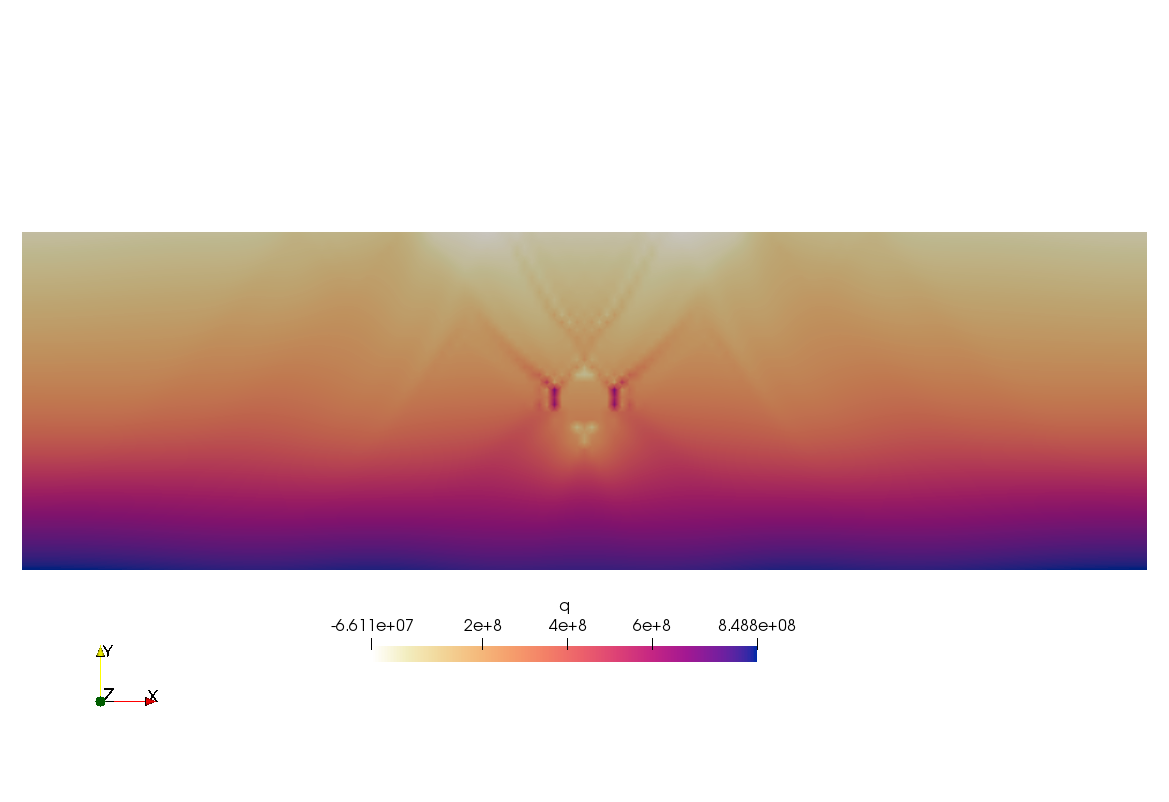
\includegraphics[width=7cm]{python_codes/fieldstone_70/extension/q}\\
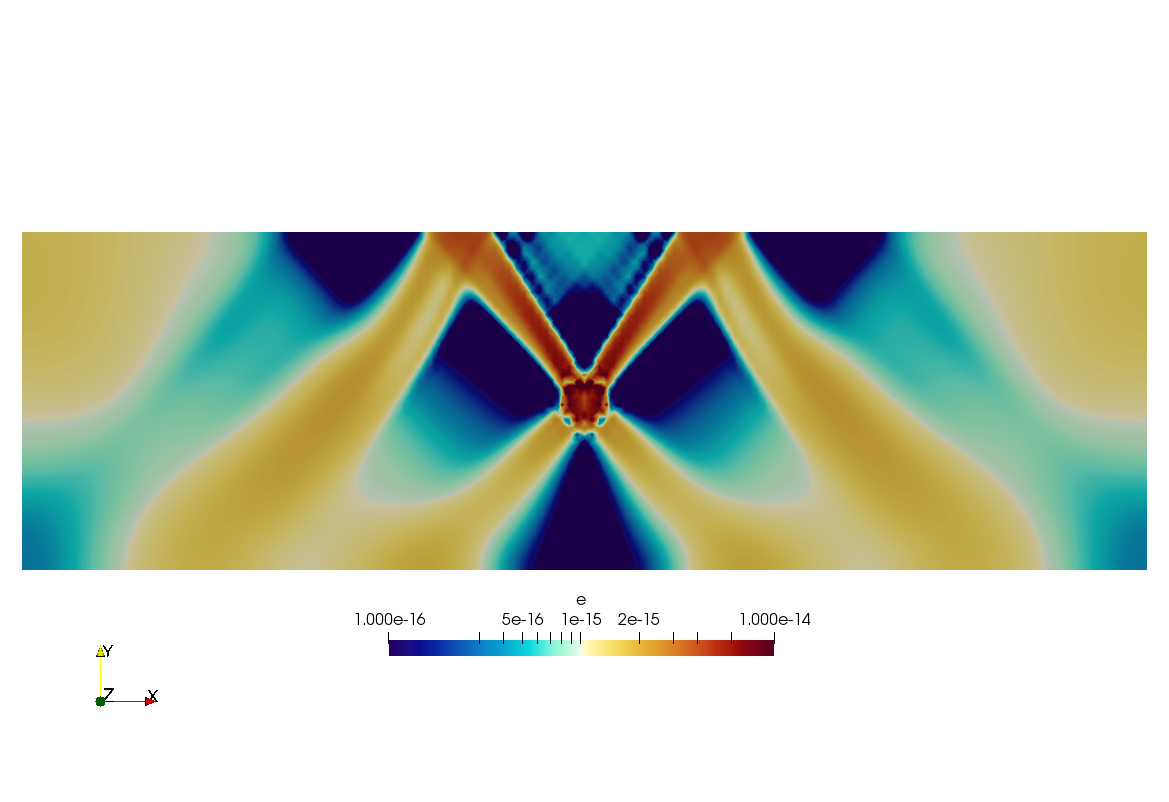
\includegraphics[width=7cm]{python_codes/fieldstone_70/extension/e}
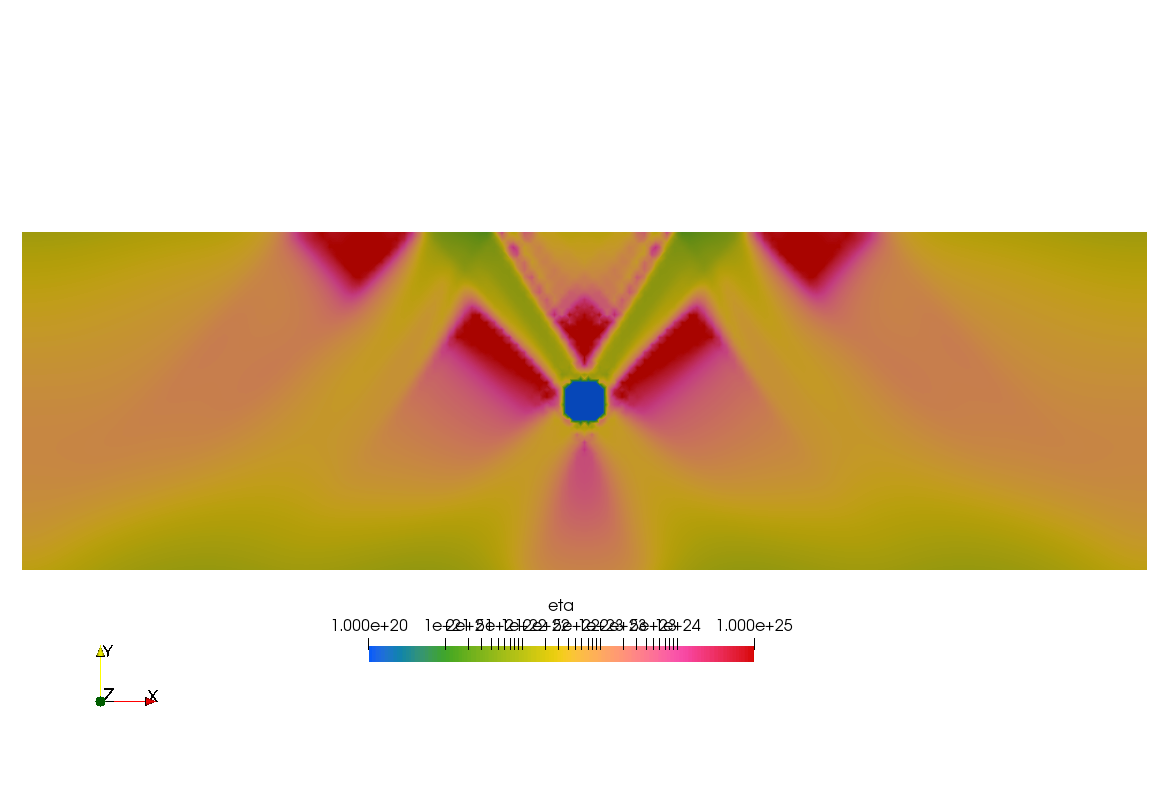
\includegraphics[width=7cm]{python_codes/fieldstone_70/extension/etaeff}\\
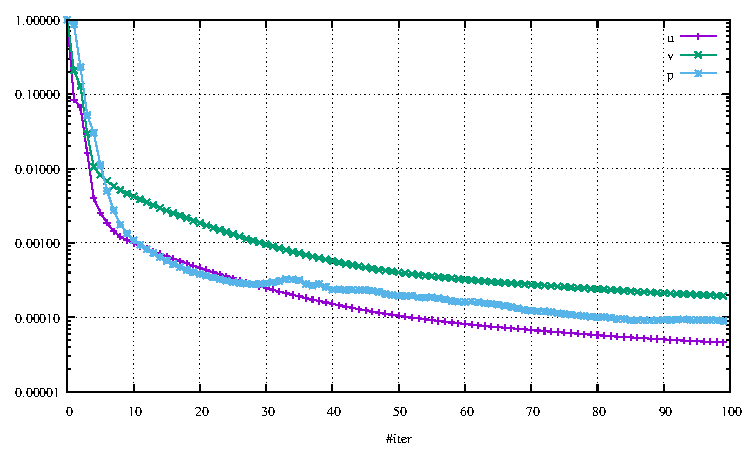
\includegraphics[width=6cm]{python_codes/fieldstone_70/extension/conv.pdf}
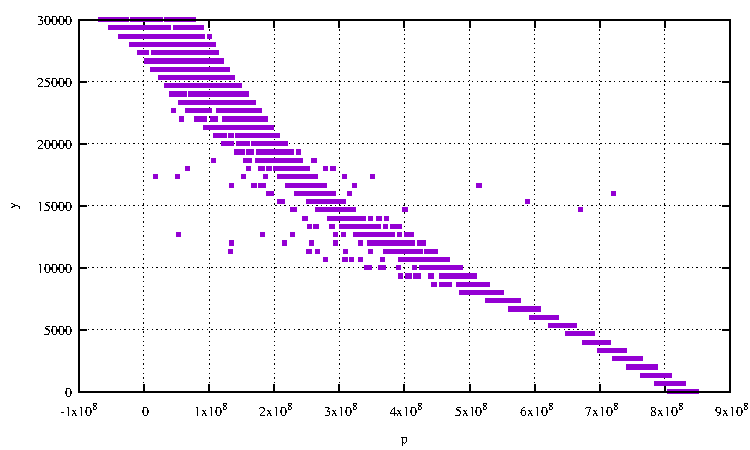
\includegraphics[width=6cm]{python_codes/fieldstone_70/extension/pressure.pdf}\\
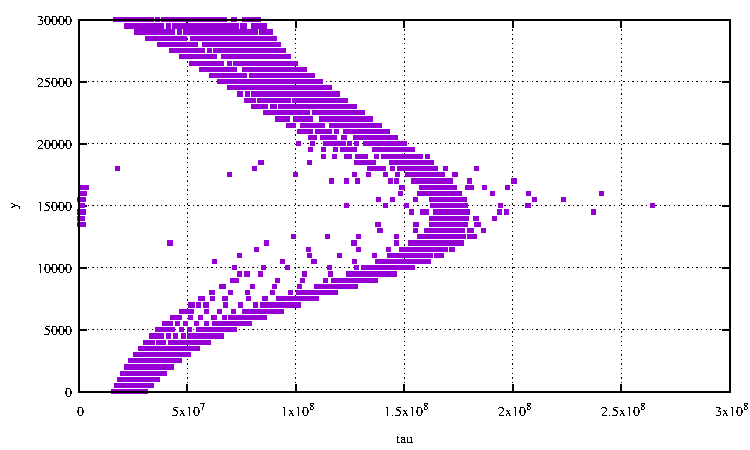
\includegraphics[width=6cm]{python_codes/fieldstone_70/extension/tau.pdf}\\
extension, resolution 150x45, 100 nl iterations only.
\end{center}

\newpage
%......................
\paragraph{Compression}.

\begin{center}
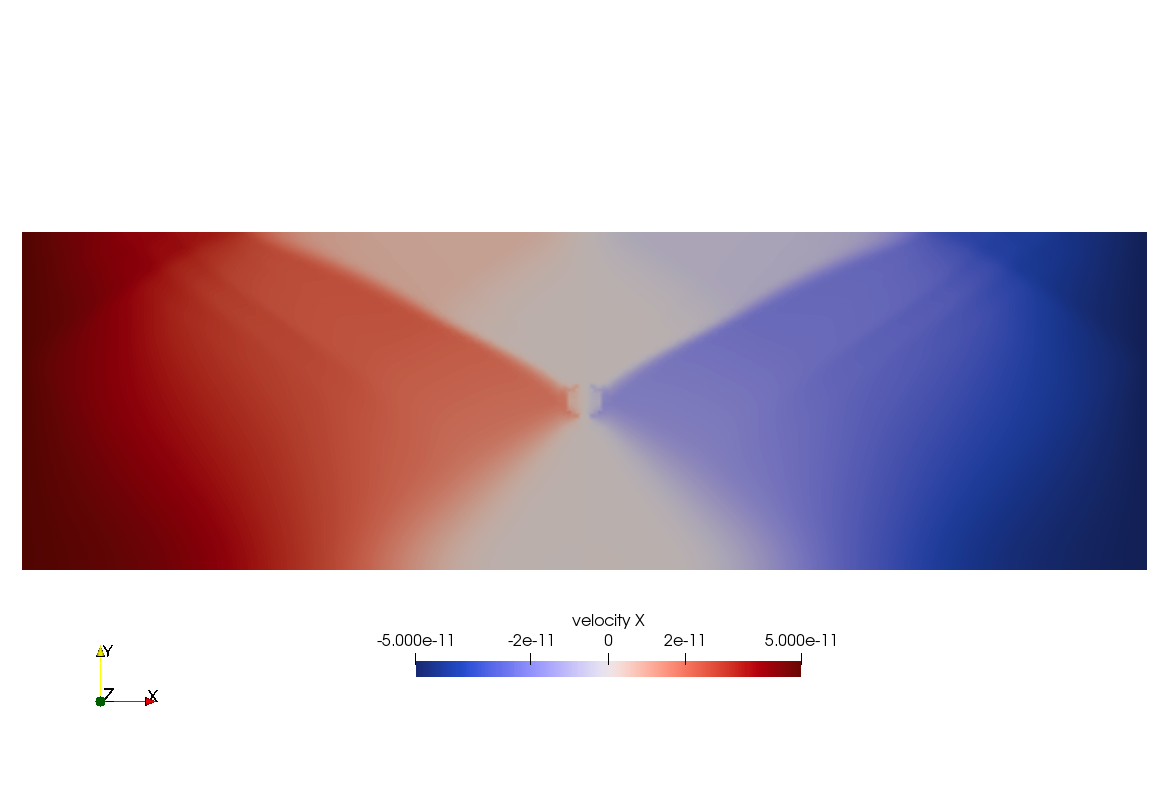
\includegraphics[width=7cm]{python_codes/fieldstone_70/compression/u}
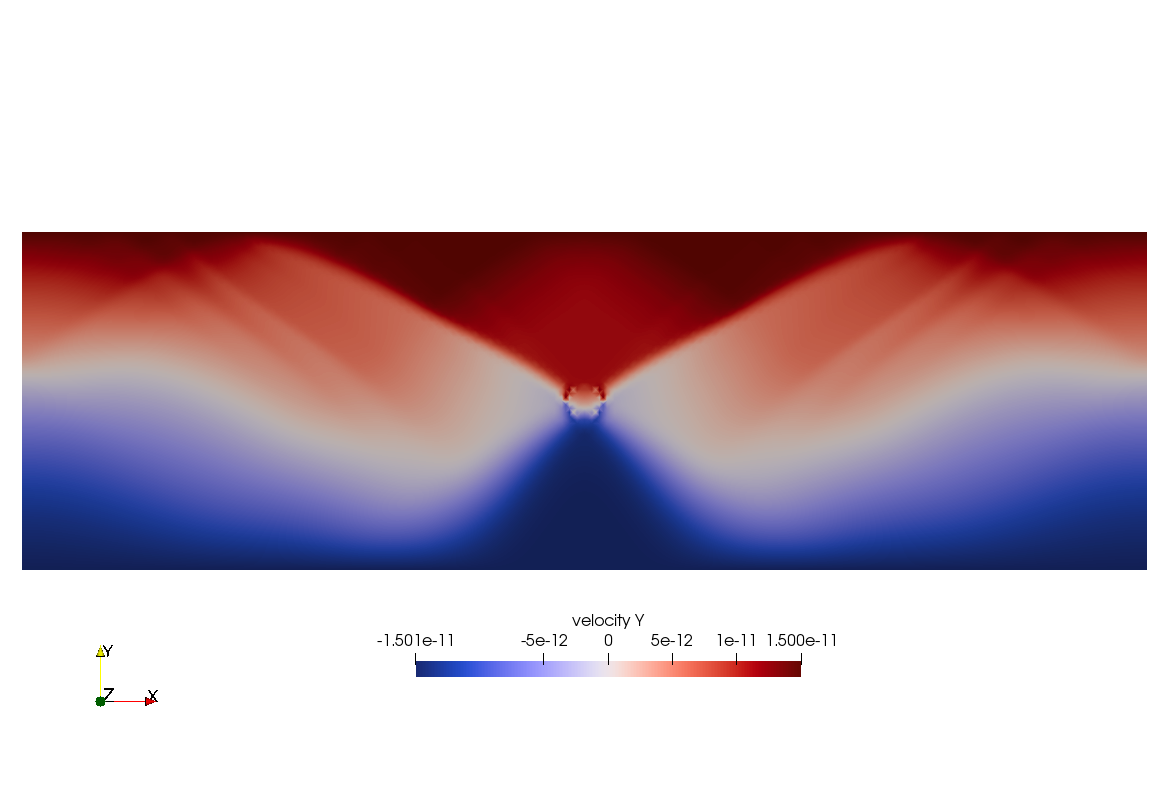
\includegraphics[width=7cm]{python_codes/fieldstone_70/compression/v}\\
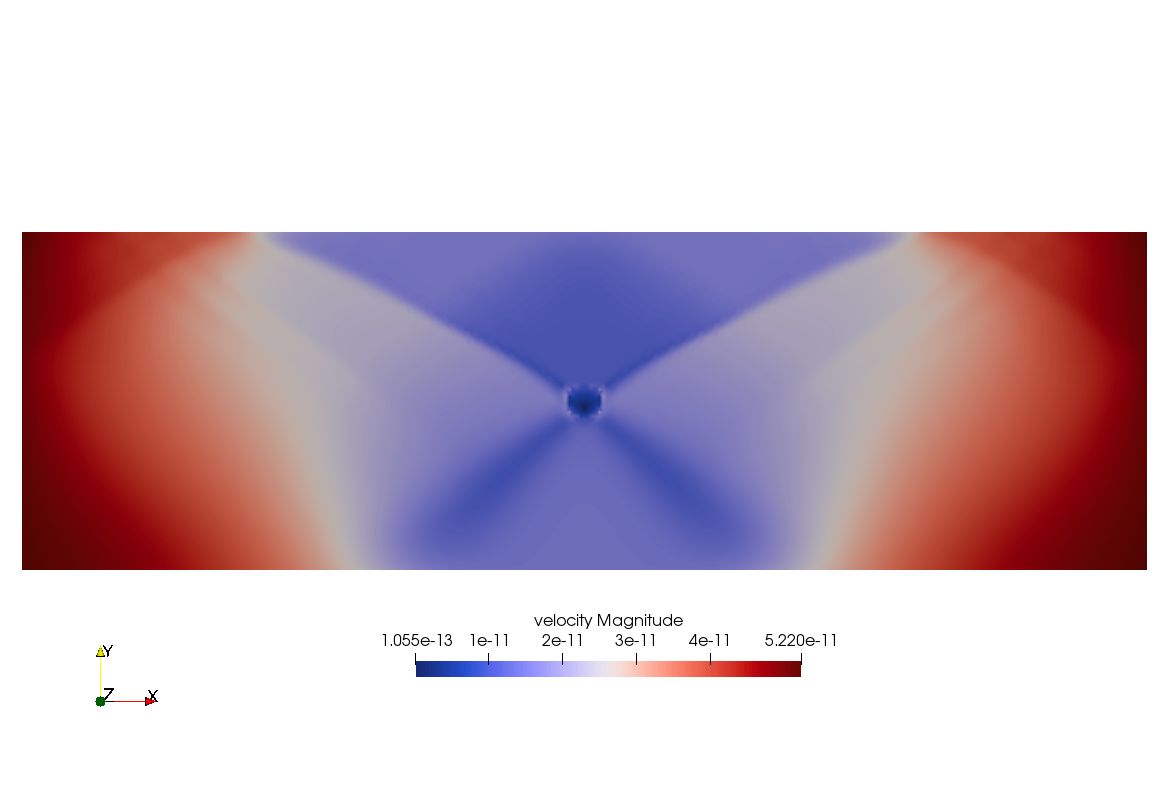
\includegraphics[width=7cm]{python_codes/fieldstone_70/compression/vel}
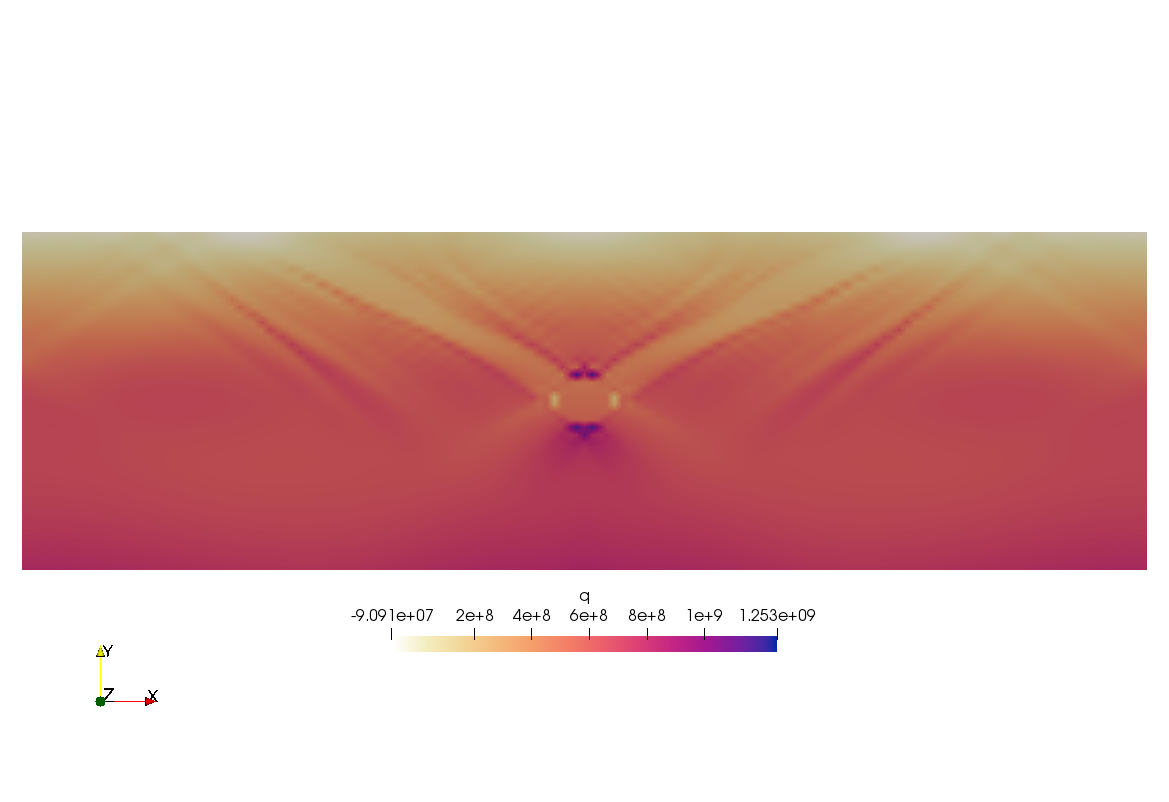
\includegraphics[width=7cm]{python_codes/fieldstone_70/compression/q}\\
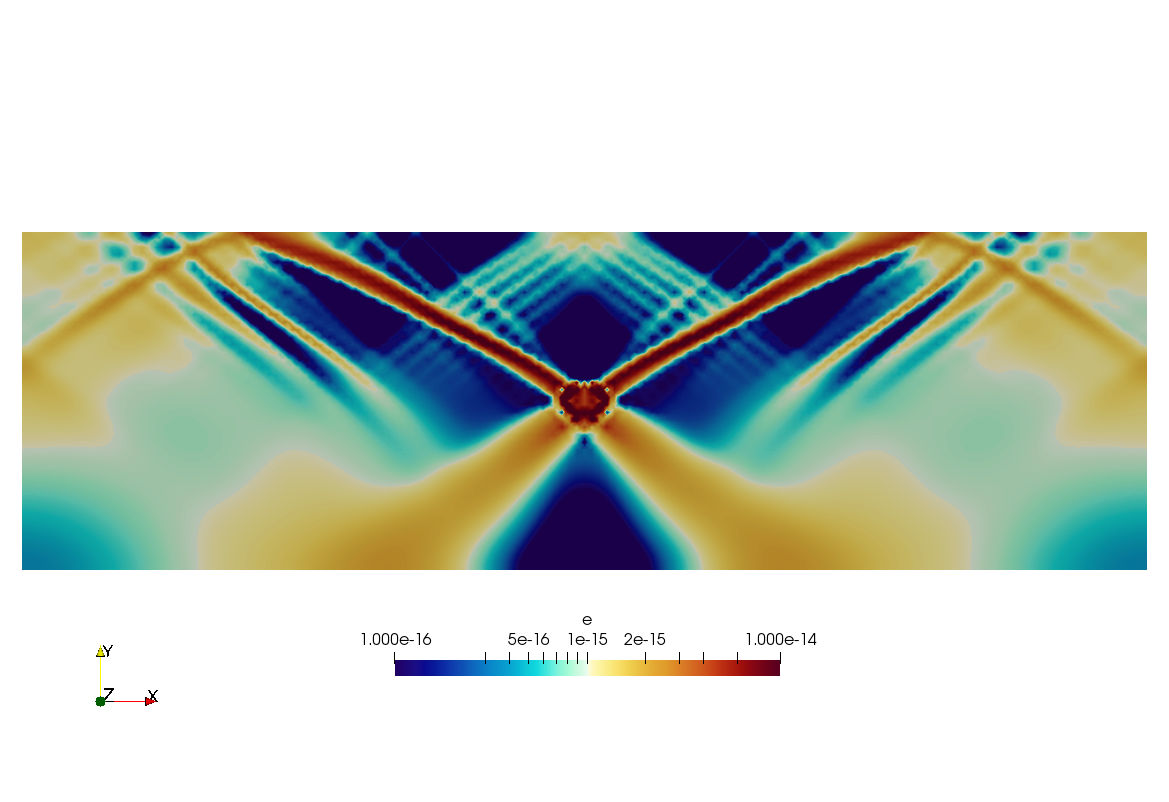
\includegraphics[width=7cm]{python_codes/fieldstone_70/compression/e}
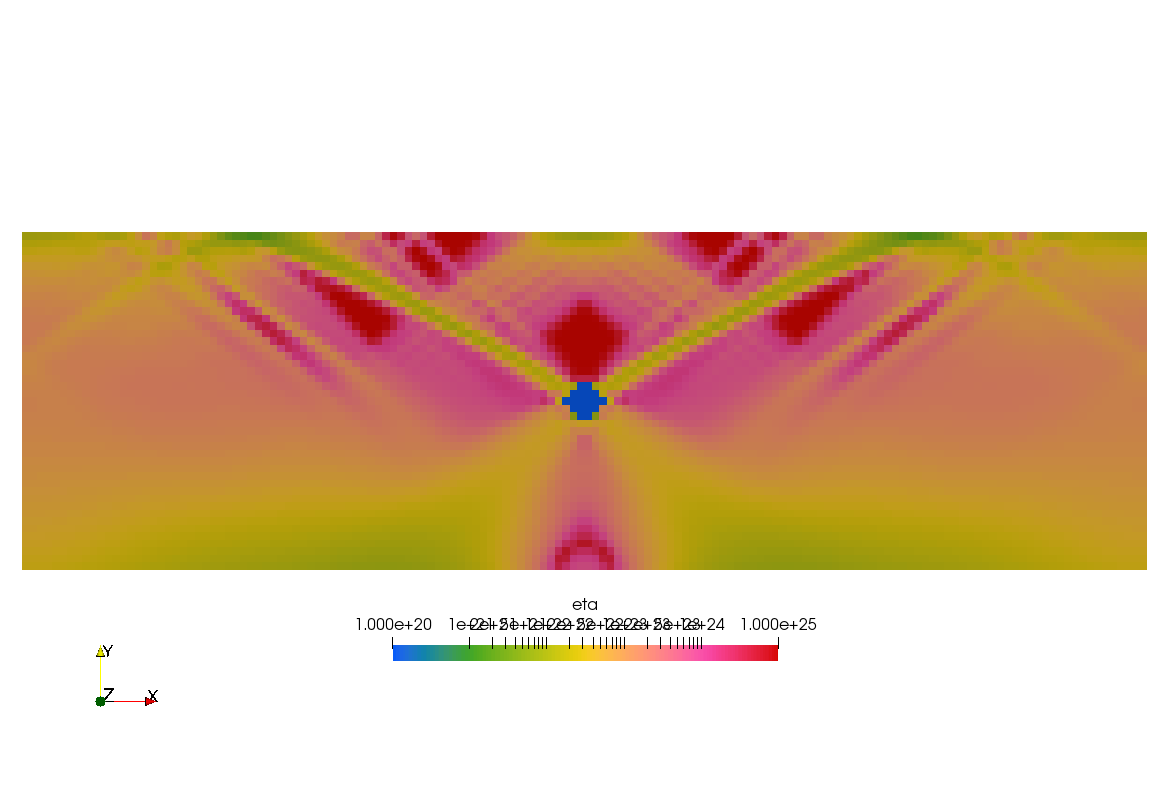
\includegraphics[width=7cm]{python_codes/fieldstone_70/compression/etaeff}\\
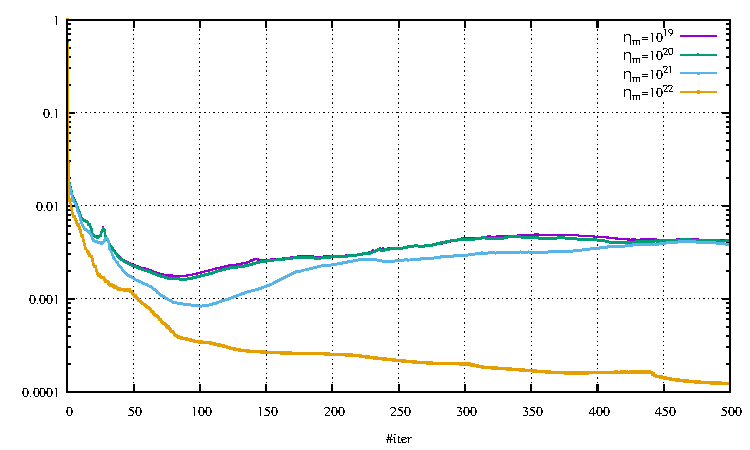
\includegraphics[width=6cm]{python_codes/fieldstone_70/compression/conv.pdf}
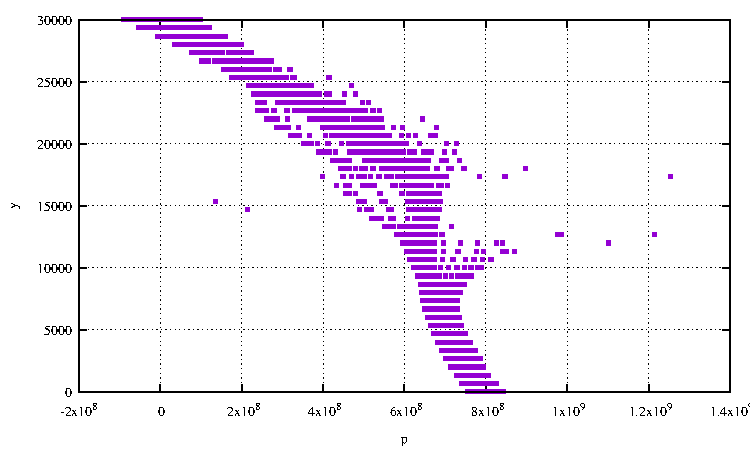
\includegraphics[width=6cm]{python_codes/fieldstone_70/compression/pressure.pdf}\\
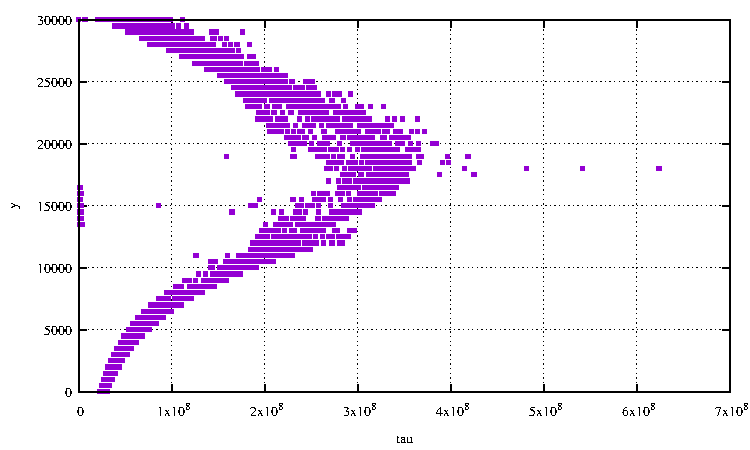
\includegraphics[width=6cm]{python_codes/fieldstone_70/compression/tau.pdf}\\
extension, resolution 150x45, 100 nl iterations only.
\end{center}

\newpage
Study of $\eta_{vp}$. 

\begin{center}
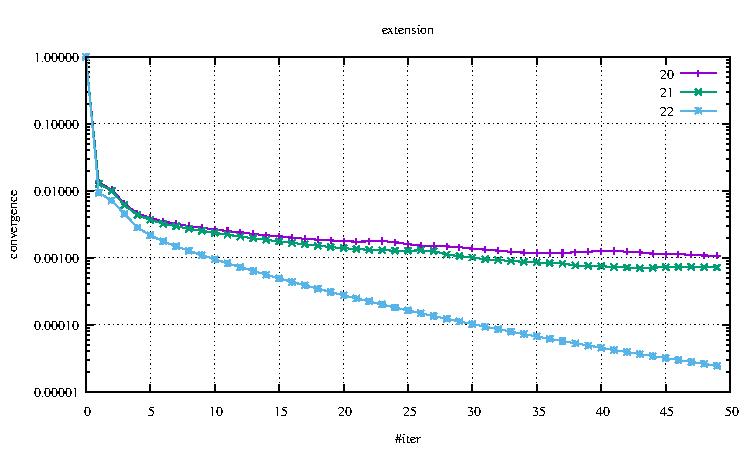
\includegraphics[width=7cm]{python_codes/fieldstone_70/results_vpstudy/conv_extension.pdf}
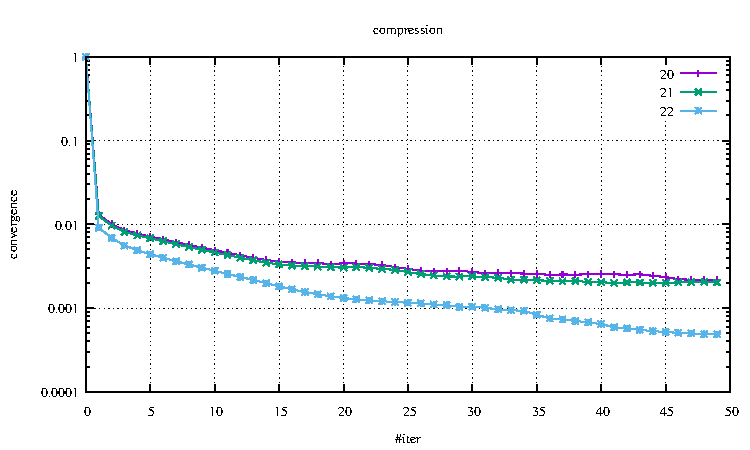
\includegraphics[width=7cm]{python_codes/fieldstone_70/results_vpstudy/conv_compression.pdf}\\
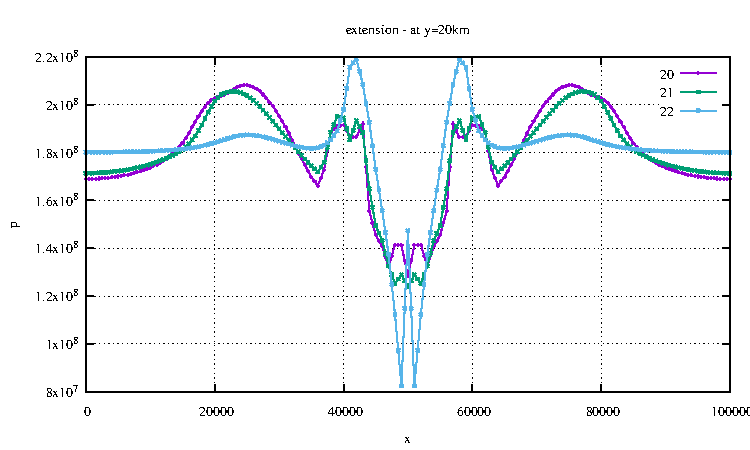
\includegraphics[width=7cm]{python_codes/fieldstone_70/results_vpstudy/pressure_extension.pdf}
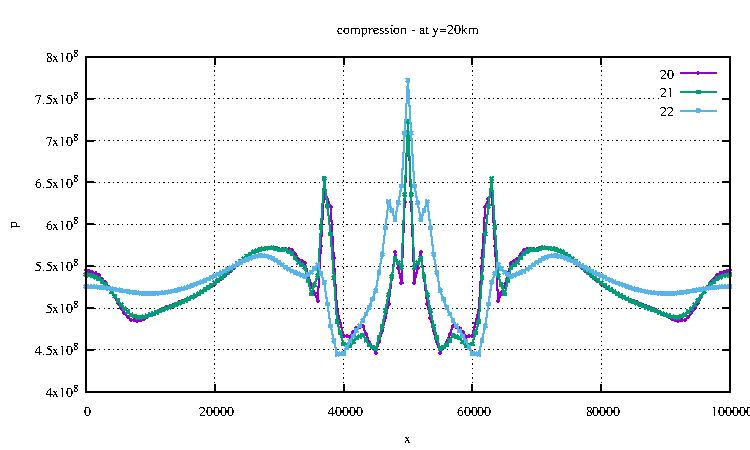
\includegraphics[width=7cm]{python_codes/fieldstone_70/results_vpstudy/pressure_compression.pdf}\\
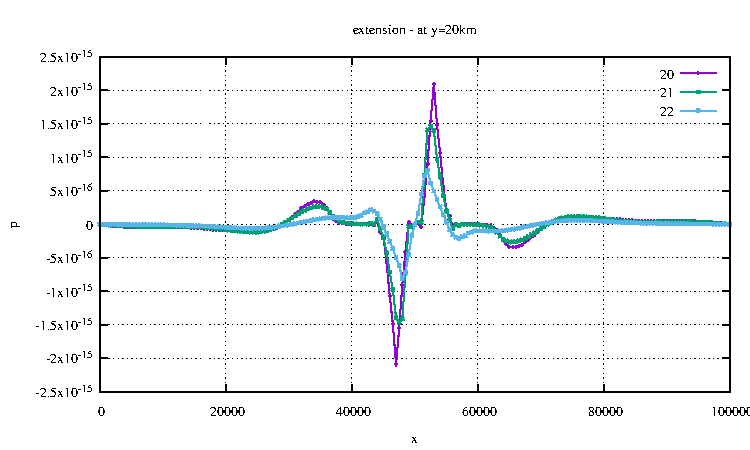
\includegraphics[width=7cm]{python_codes/fieldstone_70/results_vpstudy/exy_extension.pdf}
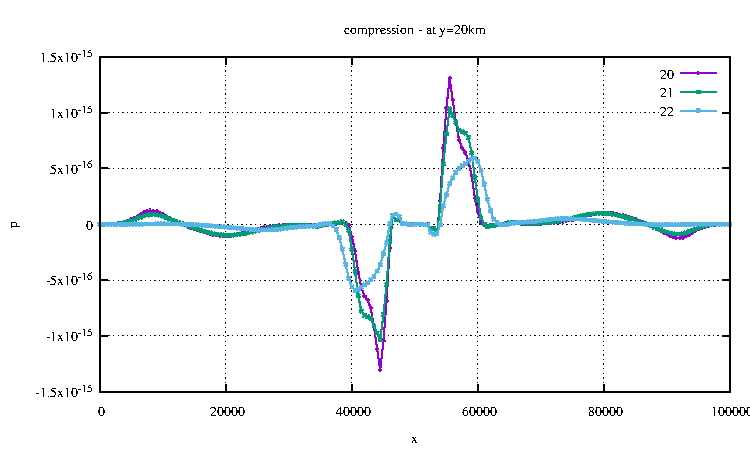
\includegraphics[width=7cm]{python_codes/fieldstone_70/results_vpstudy/exy_compression.pdf}\\
\end{center}




